\documentclass[10pt]{beamer}

\newif\ifshowarchive
\showarchivetrue   % Change to \showarchivefalse to hide archived slides

\usetheme[progressbar=frametitle]{metropolis}
\usepackage{appendixnumberbeamer}

\usepackage{booktabs}
\usepackage[scale=2]{ccicons}

\usepackage{braket}
\usepackage{twemojis}

\usepackage{pgfplots}
\usepgfplotslibrary{dateplot}
\usepackage[font=scriptsize,labelfont=bf]{caption}

\usepackage{tikz}
\usetikzlibrary{fit,shapes,positioning,calc,shapes.geometric,backgrounds}
\colorlet{tempGray}{gray!80!cyan}
\colorlet{lightgray}{tempGray!60!white}
\colorlet{orange}{red!30!yellow}
\colorlet{lightorange}{orange!60!white}
\colorlet{darkGreen}{green!80!black}
\colorlet{paleGreen}{darkGreen!30!white}

\usepackage{xspace}
\newcommand{\themename}{\textbf{\textsc{metropolis}}\xspace}

\def\code#1{\texttt{#1}}

\title{Quantum Technologies Research Project}
\subtitle{March Report}
\author{Linus Kelsey}
\date{1 Apr 26}
\institute{UCL Department of Physics and Astronomy \& \\ British Telecommunications}

\begin{document}
 
\maketitle

% ============================================================
\begin{frame}{Project Goals \& Metrics}
    \textbf{Research Gap:} No unified comparison of BB84 vs MDI-QKD across key metrics
    
    \begin{center}
        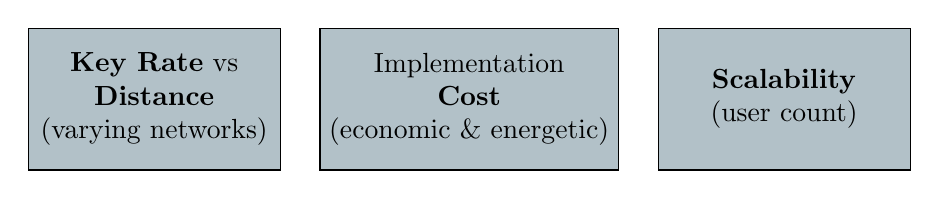
\begin{tikzpicture}
            \node[draw, fill=lightgray, minimum width=3.2cm, minimum height=1.8cm, align=center] at (0,0) {\textbf{Key Rate} vs\\\textbf{Distance}\\(varying networks)};
            \node[draw, fill=lightgray, minimum width=3cm, minimum height=1.8cm, align=center] at (4,0) {Implementation\\ \textbf{Cost}\\(economic \& energetic)};
            \node[draw, fill=lightgray, minimum width=3.2cm, minimum height=1.8cm, align=center] at (8,0) {\textbf{Scalability}\\(user count)};
        \end{tikzpicture}
    \end{center}
        
    \begin{itemize}
        \item Analyse both protocols across varying network topologies
        \item Identify parameter regimes \& topologies where each excels
        \item Inform practical QKD deployment decisions
    \end{itemize}
\end{frame}

% ============================================================
\begin{frame}{Recap: Where We Were}
    \begin{center}
        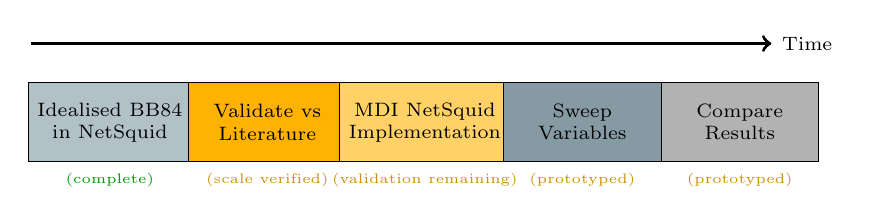
\begin{tikzpicture}[every node/.style={font=\scriptsize, align=center}]
            % Time arrow
            \draw[->, very thick] (0,1) -- (9.4,1) node[right] {Time};
            
            % Stage boxes - equal width (2cm each), positioned edge-to-edge
            \node[draw, fill=lightgray, minimum width=2cm, minimum height=1cm] (BB84) 
                at (1,0) {Idealised BB84\\in NetSquid};
            \node[draw, fill=orange, minimum width=2cm, minimum height=1cm] (validate) 
                at (3,0) {Validate vs\\Literature};
            \node[draw, fill=lightorange, minimum width=2cm, minimum height=1cm] (MDI) 
                at (5,0) {MDI NetSquid\\Implementation};
            \node[draw, fill=tempGray, minimum width=2cm, minimum height=1cm] (sweep) 
                at (7,0) {Sweep\\Variables};
            \node[draw, fill=gray!60, minimum width=2cm, minimum height=1cm] (comparison) 
                at (9,0) {Compare\\Results};

            % Status
            \node[font=\tiny, text=green!60!black, below=0.01cm of BB84] {(complete)};
            \node[font=\tiny, text=orange!80!black, below=0.01cm of MDI] {(validation remaining)};
            \node[font=\tiny, text=orange!80!black, below=0.01cm of validate] {(scale verified)};
            \node[font=\tiny, text=orange!80!black, below=0.01cm of sweep] {(prototyped)};
            \node[font=\tiny, text=orange!80!black, below=0.01cm of comparison] {(prototyped)};
        \end{tikzpicture}
    \end{center}
    
    \vspace{0.2cm}
    
    \textbf{Implementation stages:}
    \begin{enumerate}
        \item \textcolor{green!60!black}{Finalise BB84 implementation in NetSquid}
        \item \textcolor{orange!80!black}{Validate} against known rate-distance curves from literature
        \item \textcolor{green!60!black}{Adjust BB84 → MDI-QKD with symmetric setup} (+ validate)
        \item \textbf{Sweep \textcolor{orange!80!black}{distances}, topologies and scale}
        \item \textbf{Comparative analysis} across \textcolor{orange!80!black}{metrics}
    \end{enumerate}
\end{frame}

% ============================================================
\begin{frame}{Since last meeting}
    \textbf{March Progress}
    \begin{itemize}\small
        \item Loss model: Beer-Lambert $T = 10^{-\alpha L/10}$ implemented
        \item Detector efficiency model implemented
        \item Three comparative sweep graphs produced
        \item Literature Review submitted
    \end{itemize}
    \vspace{0.3cm}
    \textbf{Action list}
    \begin{itemize}\small
        \item Relative \emph{and} absolute key rate scales + MDI duplicated distance\hfill\twemoji{check mark button}
        \item Effect of BB84 repeaters on comparison \hfill\twemoji{hourglass not done}
        \item Vary Charlie's location \hfill\twemoji{hourglass not done}
        \item Practical key rate thresholds \hfill\twemoji{hourglass not done}
        \item One-pager: modelling plan \& layering inc. MDI synchronisation\hfill\twemoji{hourglass not done}
    \end{itemize}
\end{frame}
 
% ============================================================
\begin{frame}{Modelling Status: Layered Build-up}
    \vspace{0.5cm}
    \begin{center}
    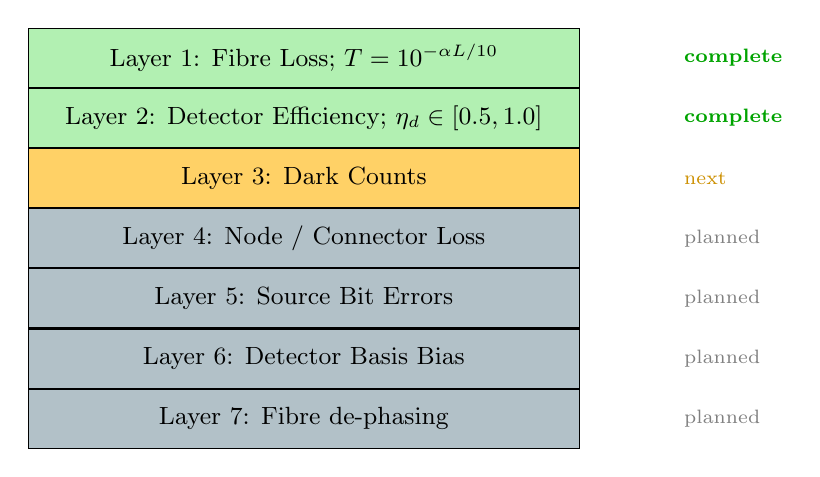
\begin{tikzpicture}[every node/.style={font=\small, align=center}, node distance=0.5cm]
        \node[draw, fill=darkGreen!30!white, minimum width=7cm, minimum height=0.75cm] (L1)
            {Layer 1: Fibre Loss; $T = 10^{-\alpha L / 10}$};
        \node[draw, fill=darkGreen!30!white, minimum width=7cm, minimum height=0.75cm, below=0cm of L1] (L2)
            {Layer 2: Detector Efficiency; $\eta_d \in [0.5, 1.0]$};
        \node[draw, fill=lightorange, minimum width=7cm, minimum height=0.75cm, below=0cm of L2] (L3)
            {Layer 3: Dark Counts};
        \node[draw, fill=lightgray, minimum width=7cm, minimum height=0.75cm, below=0cm of L3] (L4)
            {Layer 4: Node / Connector Loss};
        \node[draw, fill=lightgray, minimum width=7cm, minimum height=0.75cm, below=0cm of L4] (L5)
            {Layer 5: Source Bit Errors};
        \node[draw, fill=lightgray, minimum width=7cm, minimum height=0.75cm, below=0cm of L5] (L6)
            {Layer 6: Detector Basis Bias};
        \node[draw, fill=lightgray, minimum width=7cm, minimum height=0.75cm, below=0cm of L6] (L7)
            {Layer 7: Fibre de-phasing};
 
        \node[right=1.2cm of L1, font=\scriptsize, text=darkGreen!80!black] {\textbf{complete}};
        \node[right=1.2cm of L2, font=\scriptsize, text=darkGreen!80!black] {\textbf{complete}};
        \node[right=1.2cm of L3, font=\scriptsize, text=orange!80!black] {next};
        \node[right=1.2cm of L4, font=\scriptsize, text=gray] {planned};
        \node[right=1.2cm of L5, font=\scriptsize, text=gray] {planned};
        \node[right=1.2cm of L6, font=\scriptsize, text=gray] {planned};
        \node[right=1.2cm of L7, font=\scriptsize, text=gray] {planned};
    \end{tikzpicture}
    \end{center}
    \vspace{0.2cm}
    \footnotesize
    \textbf{Note:} Error correction and privacy amplification are \emph{not} planned - both protocols use identical methods, so omitting them preserves fairness of comparison at the physical layer.
\end{frame}

% ============================================================
\begin{frame}{Results I: Key Rate vs Fibre Attenuation Rate}
    \begin{columns}[T]
        \column{55mm}
            \vspace{0.2cm}
            \small
            \begin{itemize}
                \item Fixed: 50 km Alice--Bob distance, $\eta_d = 0.9$
                \item Both curves \textbf{linear on log scale} $\Rightarrow$ exponential decay in rate with attenuation
                \item MDI offset below BB84 by $\approx$\,constant factor across all $\alpha$
                \item Offset consistent with 50\% BSM efficiency cap and $\eta_d^2$ dependence
                \item At $\alpha = 0.2$\,dB/km (standard SMF): BB84 $\approx 70$\,kbps, MDI $\approx 25$\,kbps
                \item Both remain operationally viable across commercial attenuation range
            \end{itemize}
        \column{58mm}
            \begin{figure}
                \centering
                \frame{
\includegraphics[width=\linewidth]{images/kr_v_loss_001.png}}
                \caption{Key rate vs fibre attenuation. 50 km, $\eta_d = 0.9$.}
            \end{figure}
    \end{columns}
\end{frame}
 
% ============================================================
\begin{frame}{Results II: Key Rate vs Distance}
    \begin{columns}[T]
        \column{55mm}
            \vspace{0.4cm}
            \small
            \begin{itemize}
                \item Fixed: $\alpha = 0.2$\,dB/km, $\eta_d = 0.9$
                \item BB84 and MDI both show near-linear decay on log scale at long distances
                \item MDI decays \textbf{faster}: gap widens beyond $\sim\!30$\,km
                \item At 100 km: BB84 $\sim\!4$\,kbps, MDI $\sim\!2$\,kbps
                \item Crossover not observed in this range
            \end{itemize}
        \column{58mm}
            \begin{figure}
                \centering
                \frame{
\includegraphics[width=\linewidth]{images/kr_v_distance_001.png}}
                \caption{Key rate vs Alice--Bob separation. $\alpha = 0.2$\,dB/km, $\eta_d = 0.9$.}
            \end{figure}
    \end{columns}
\end{frame}
 
% ============================================================
\begin{frame}{Results III: Key Rate vs Detector Efficiency}
    \begin{columns}[T]
        \column{58mm}
            \vspace{0.2cm}
            \small
            \begin{itemize}
                \item Fixed: 50 km, $\alpha = 0.2$\,dB/km
                \item BB84 degrades \textbf{slowly}: near-linear in $\eta_d$, losing $\sim\!50\%$ from $\eta_d = 1 \to 0.5$
                \item MDI degrades \textbf{quadratically}: losing $\sim\!90\%$ over the same range
                \item MDI depends on coincident detection at two detectors
                \item \textbf{Practical implication:} MDI is strongly penalised by imperfect detectors
                \item SNSPDs ($\eta_d \approx 0.9\text{--}0.95$) are therefore \emph{not} optional for MDI
            \end{itemize}
        \column{58mm}
            \begin{figure}
                \centering
                \frame{
\includegraphics[width=\linewidth]{images/kr_v_eff_001.png}}
                \caption{Key rate vs detector efficiency. 50 km, $\alpha = 0.2$\,dB/km.}
            \end{figure}
    \end{columns}
\end{frame}
 
% ============================================================
\begin{frame}{Discussion: Fairness of Comparison}
    \vspace{0.3cm}
    \textbf{Concurrent question:} Are MDI and BB84 being compared like for like?
 
    \begin{center}
    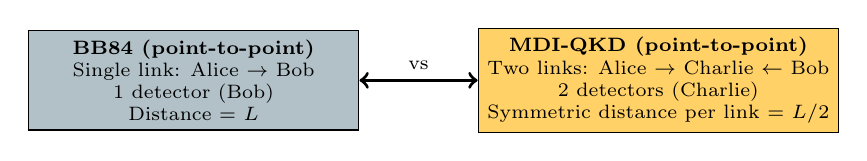
\begin{tikzpicture}[every node/.style={font=\scriptsize, align=center}, node distance=0.4cm]
        \node[draw, fill=lightgray, minimum width=4.2cm, minimum height=1.2cm] (bb84)
            {\textbf{BB84 (point-to-point)}\\Single link: Alice $\to$ Bob\\1 detector (Bob)\\Distance = $L$};
        \node[draw, fill=lightorange, minimum width=4.2cm, minimum height=1.2cm, right=1.5cm of bb84] (mdi)
            {\textbf{MDI-QKD (point-to-point)}\\Two links: Alice $\to$ Charlie $\leftarrow$ Bob\\2 detectors (Charlie)\\Symmetric distance per link = $L/2$};
        \draw[<->, very thick] (bb84.east) -- (mdi.west) node[midway, above, font=\scriptsize] {vs};
    \end{tikzpicture}
    \end{center}
    \vspace{0.2cm}
    \begin{itemize}
        \item Current: BB84 and MDI use identical Alice--Bob separation $L$, and \textbf{all sources and detectors are the same}
        \item MDI disadvantage in rate arises from: (1) 50\% BSM efficiency cap, (2) $\eta_d^2$ at Charlie's two detectors
        \item Greatest effect on key rate decay (for both) is fibre attenuation - \textbf{3 orders of magnitude} drop-off from 1 to 100 km.
        \item Constant ratio exhibited for distance and attenuation - detector efficiency causes a \textbf{linear increase in gap} between BB84 and MDI
    \end{itemize}
\end{frame}
 
% ============================================================
\begin{frame}{Next Steps}
    \textbf{Simulation priorities (June):}
    \begin{itemize}
        \item Dark count model: scale $d_c$ proportionally with detection rate; sensitivity analysis on $d_c/\eta$ ratio
        \item Build in further modelling parameters
        \item Begin validation: match absolute key rate curves
        \item Start work extending to network-scale simulation
    \end{itemize}
 
    \vspace{0.15cm}
    \textbf{Analysis priorities:}
    \begin{itemize}
        \item Modelling proposal - device and network parameters
        \item Identify QBER threshold crossings ($>11\%$) as a function of distance, loss, and $\eta_d$ for trusted node analysis
        \item Assess whether Charlie's position affects performance
    \end{itemize}
\end{frame}

% ============================================================
\begin{frame}{Timeline}
    \begin{center}
    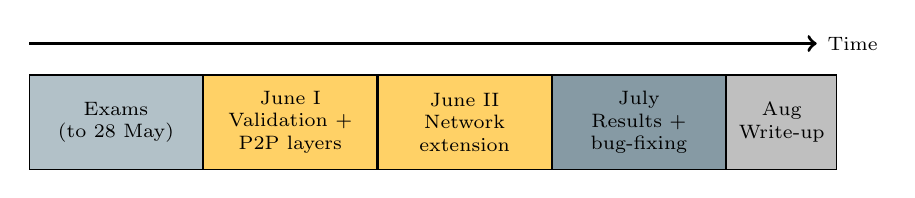
\begin{tikzpicture}[every node/.style={font=\scriptsize, align=center}]
        \draw[->, very thick] (0,1) -- (10,1) node[right] {Time};
 
        \node[draw, fill=lightgray, minimum width=2.2cm, minimum height=1.2cm] (exams) at (1.1, 0)
            {Exams\\(to 28 May)};
        \node[draw, fill=lightorange, minimum width=2.2cm, minimum height=1.2cm, right=0cm of exams] (june1) 
            {June I\\Validation +\\P2P layers};
        \node[draw, fill=lightorange, minimum width=2.2cm, minimum height=1.2cm, right=0cm of june1] (june2) 
            {June II\\Network\\extension};
        \node[draw, fill=tempGray, minimum width=2.2cm, minimum height=1.2cm, right=0cm of june2] (july) 
            {July\\Results +\\bug-fixing};
        \node[draw, fill=gray!50, minimum width=1.4cm, minimum height=1.2cm, right=0cm of july] 
            {Aug\\Write-up};
    \end{tikzpicture}
    \end{center}
    \vspace{0.1cm}
    \small
    \begin{itemize}
        \item \textbf{June first half:} Validation benchmarking (BB84 + MDI); complete P2P modelling layers (dark counts $\to$ node loss $\to$ beyond)
        \item \textbf{June second half:} Begin network-scale extension; trusted node BB84 vs MDI comparison
        \item \textbf{July:} Inevitable bug-catching, parameter sweeps, result collection
        \item \textbf{August:} Write-up, final figures, submission preparation; submission
        \item \textbf{September:} Viva
    \end{itemize}
\end{frame}
 
\end{document}
